\section{Viewpoint Skew: Definitions and Theory}
\label{sec:framework}

A cocoon is not a property of any single video. It is a relation between the mix of videos a person is shown and some reference mix. This section fixes the quantities we measure and derives what user actions can do to them: \cref{sec:coords} describes a feed by two coordinates, \cref{sec:layers} splits its skew into a platform and a personal layer, \cref{sec:actions} derives how feedback, topic controls and filters move a feed, and \cref{sec:notice} bounds what a user can detect. \Cref{sec:formation,sec:detection,sec:escape} test or apply the propositions; proofs are in \cref{app:proofs}.

\subsection{Two coordinates of a feed}
\label{sec:coords}

Let $\I$ be the set of all videos and $\I_k\subseteq\I$ those about issue $k$, here gender and marriage. Within the issue, a \emph{target narrative} $\A\subseteq\I_k$ (videos that attach a negative label to a whole gender) is set against the \emph{retained set} $\B=\I_k\setminus\A$, the rest of the topic, which the user wants to keep. For user $u$, let $\pi_u(i)$ be the probability that the next video shown is $i$, and write $\pi_u(G)=\sum_{i\in G}\pi_u(i)$.

\begin{definition}[State of a feed]
The \emph{topic share} and the \emph{within-issue share} of user $u$ are
\begin{equation}
  m_u=\pi_u(\I_k),\qquad p_u=\frac{\pi_u(\A)}{\pi_u(\I_k)} .
\end{equation}
\end{definition}

The topic share measures interest. The within-issue share measures what the user meets once on the topic. Category-diversity measures are functions of topic shares alone: they can tell how much of a feed is about the issue, but not what the user meets within it. Two users with the same $m_u$ may differ arbitrarily in $p_u$, as the two feeds of \cref{fig:teaser} do.

\subsection{Three layers of skew}
\label{sec:layers}

Whether $p_u$ is high depends on the reference. We use two: the \emph{supply share} $\psup$, the fraction of distinct issue videos on the platform that belong to $\A$, and the \emph{platform share} $\pbar=\bar\pi(\A)/\bar\pi(\I_k)$, where $\bar\pi$ averages exposure over all users. On the log-odds scale, $\logit p=\log\frac{p}{1-p}$, the skew a user experiences relative to supply splits exactly:
\begin{equation}
  \underbrace{\logit p_u-\logit\psup}_{\text{total skew}}
  \;=\;\underbrace{\logit\pbar-\logit\psup}_{\text{platform layer }\Lambda}
  \;+\;\underbrace{\logit p_u-\logit\pbar}_{\text{personal layer }V_u}.
  \label{eq:decomp}
\end{equation}

\begin{definition}[Viewpoint skew]
The \emph{viewpoint skew} of user $u$ is the personal layer $V_u=\logit p_u-\logit\pbar$. A user is in a \emph{viewpoint cocoon} when $V_u$ is large, whatever the value of $m_u$.
\end{definition}

The platform layer $\Lambda$ is shared by everyone: ranking that favours a narrative raises it in all feeds. The personal layer is what personalisation adds for one user. Supply is described and not judged, since calling supply itself ``skewed'' would need an outside standard, such as the distribution of views in society, which we do not have. We assume that a feed without personalisation shows the narrative at the platform share $\pbar$; $V_u$ is then also the user's skew relative to what they would see with personalisation switched off. With the values measured in \cref{sec:platform,sec:logs}, group-label videos are 4.1\% of the marriage videos on offer and 6.2\% of those shown, and a user in the most skewed tenth of heavy viewers sees \nTopDecileShare\%. Reporting $V_u$ alone would hide that the platform already shows the narrative 1.5 times as often as supply; reporting the total alone would hide that personalisation more than doubles the odds again.


\begin{figure}[t]
  \centering
  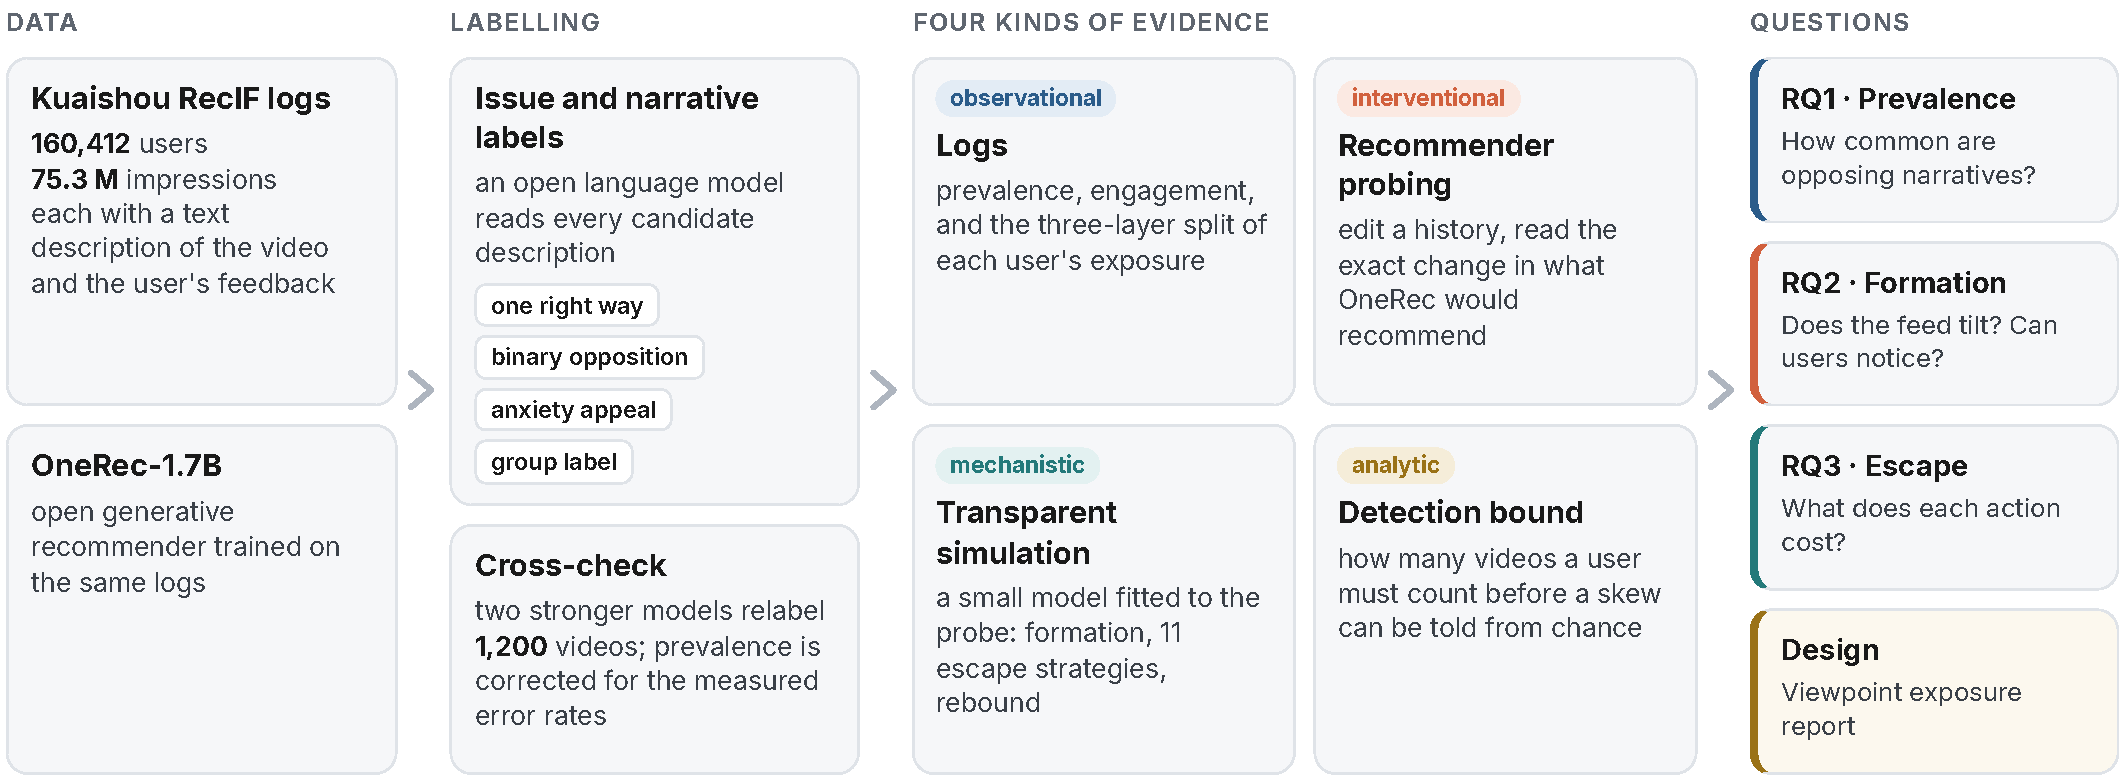
\includegraphics[width=\textwidth]{figures/fig_overview.pdf}
  \caption{Study design. \textbf{\cnum{1} Data:} Kuaishou's public RecIF logs record what 160{,}412 users were shown and how they reacted; OneRec, trained on the same logs, reads a history of semantic video IDs and scores candidate videos. \textbf{\cnum{2} Labelling:} a screen narrows the logs to candidate videos, an open model labels each one by domain, narrative type and the four-part group-label rule, and two stronger models check a sample of 1{,}200. \textbf{\cnum{3} Evidence:} the logs describe what users were shown; probes edit histories given to OneRec and read the change in its scores; a transparent simulation, whose recommender is fitted to the probes, follows users for months; and a statistical bound says how many videos a user would have to count. \textbf{\cnum{4} Questions:} each kind of evidence answers the research questions marked on it.}
  \label{fig:overview}
\end{figure}

\subsection{How user actions move the state}
\label{sec:actions}

To reason about actions we use the standard form of a learned recommender. Each video has a vector $v_i$ and a baseline weight $q_i>0$ set by global ranking, user $u$ has a state vector $x_u$ learned from their history, and
\begin{equation}
  \pi_u(i)\;\propto\;q_i\,\exp\langle x_u,v_i\rangle .
  \label{eq:softmax}
\end{equation}
Feedback on video $j$ moves the state to $x_u+\eta v_j$, with $\eta>0$ if the system reads the feedback as interest and $\eta<0$ if it reads it as rejection. Let $s_j(i)=\langle v_j,v_i\rangle$ and let $\bar s_j(G)$ be its exposure-weighted mean over a set $G$.

\begin{proposition}[First-order effect of feedback]
\label{prop:feedback}
For small $\eta$, feedback on video $j$ changes the state by
\begin{equation}
  \Delta V=\eta\,c_j+O(\eta^2),\qquad \Delta\logit m=\eta\,t_j+O(\eta^2),
\end{equation}
where $c_j=\bar s_j(\A)-\bar s_j(\B)$ is the \emph{narrative contrast} of $j$ and $t_j=\bar s_j(\I_k)-\bar s_j(\I\setminus\I_k)$ its \emph{topic contrast}.
\end{proposition}

Three consequences follow. \emph{First}, formation and escape depend on the same quantity. A user who finishes more $\A$ than $\B$ videos gains skew at a rate proportional to $c$; if the recommender does not separate the narrative ($c\approx0$), preferences cannot build a personal skew and feedback cannot remove one. \emph{Second}, feedback on a narrative video moves the user along a line of slope $c/t$ in the plane of $\logit m$ and $V$: each unit of skew removed by a rejection costs $t/c$ units of topic log-odds. \emph{Third}, the sign of $\eta$ for a button such as ``not interested'' is the platform's choice, not the user's.

\begin{proposition}[Topic-level controls]
\label{prop:topic}
If an action multiplies the exposure of every video in $\I_k$ by the same factor, then $\Delta V=0$. Moreover, if no content category separates $\A$ from $\B$, any statistic of a feed that depends only on category shares takes the same value on feeds that differ only in $V$.
\end{proposition}

``Show less of this topic'', switching a category off, and every cocoon check built on categories are of this kind.

\begin{proposition}[Filters]
\label{prop:filter}
Suppose a filter hides each $\A$ video with probability $\mathrm{TPR}$ and each $\B$ video with probability $\mathrm{FPR}$, and hidden slots are not refilled. Then, with the recommender's state unchanged,
\begin{equation}
  \Delta V=\log\frac{1-\mathrm{TPR}}{1-\mathrm{FPR}},
\end{equation}
and the number of issue videos the user sees falls by the factor $1-p\,\mathrm{TPR}-(1-p)\,\mathrm{FPR}$.
\end{proposition}

Keyword lists, creator blocklists and classifier-based filters differ only in these two rates. A filter acts on what reaches the screen, so it is the one user-side action whose direct effect does not depend on the recommender.

\begin{proposition}[Reach of user actions]
\label{prop:reach}
The platform layer $\Lambda$ does not depend on $x_u$. An action that returns the state to its default $x^0$ (clearing history, switching personalisation off) leaves the user with total skew $\Lambda$. A total skew below $\Lambda$ requires $V<0$, that is, either a filter or a state that encodes aversion to the narrative; in a recommender that forgets, such a state lasts only while the signals that produce it continue.
\end{proposition}

\subsection{What a user can notice}
\label{sec:notice}

A user sees only their own feed. To learn whether a narrative is over-represented, they, or a tool acting for them, must count it in what they see and compare the count with a reference sample, for example the same topic with personalisation switched off. Both counts pass through a classifier with recall $\alpha$ and false-positive rate $\beta$, so a true share $p$ is observed as $q=\beta+(\alpha-\beta)p$~\citep{rogan1978prevalence}.

\begin{proposition}[Sample size for detection]
\label{prop:detect}
A one-sided test at level $a$ with power $1-\gamma$ that the user's share exceeds the reference share $p_0$ needs, in each of the two samples,
\begin{equation}
  n\;\approx\;\frac{(z_{a}+z_{\gamma})^2\,\bigl[q_u(1-q_u)+q_0(1-q_0)\bigr]}{(\alpha-\beta)^2\,(p_u-p_0)^2}
  \label{eq:detect}
\end{equation}
issue videos, where $z$ denotes standard normal quantiles.
\end{proposition}

The platform is in a different position. It knows $\pi_u$ and can compute $V_u$ without sampling.
